%% V1.0
%% by Gabriel Garcia, gabrcg@gmail.com
%% This is a template for Udacity projects using IEEEtran.cls

%% Be Udacious!

\documentclass[10pt,journal,compsoc]{IEEEtran}

\usepackage[pdftex]{graphicx}
\usepackage{cite}
\hyphenation{op-tical net-works semi-conduc-tor}
\usepackage{hyperref}
\usepackage{listings}

\begin{document}

\title{Deep RL Arm Manipulation}

\author{Jeremy Hale}

\markboth{Robotics Nanodegree Program, Udacity}%
{}
\IEEEtitleabstractindextext{%

\begin{abstract}
Deep reinforcement learning for robotic manipulator using Gazebo.
\end{abstract}

% Note that keywords are not normally used for peerreview papers.
\begin{IEEEkeywords}
Robot, IEEEtran, Udacity, \LaTeX, Deep RL.
\end{IEEEkeywords}}

\maketitle
\IEEEdisplaynontitleabstractindextext
\IEEEpeerreviewmaketitle
\section{Introduction}
\label{sec:introduction}

\IEEEPARstart{T}{his} project uses deep reinforcement learning to train a robot arm to touch an object in simulation.

\section{Reward Function}
The reward function for the first challenge was based on the change in distance to the target. Moving towards the target yielded no reward but moving away incurred a 1 point penalty. Touching the ground yielded a large penalty of 10 points while touching the target with any part of the arm yielded 100 points.

For the second challenge, only collisions between the gripper base and the target counted as success. Also, the reward function was slightly simplified. Touching the target with the base yielded 1 point, while touching the ground yielded 0 points. The agent also received a 1 point penalty for moving away from the target, but no reward for moving closer.

The main change to the reward function for the second challenge was to fix the code for calculating distance to target. There was an error where the algorithm used the world pose of "tube" which is 0, 0, 0.075. The much more useful location is that of "tube\_link" which is 1.15, 0, 0. Surprisiginly the first challenge worked with the incorrect distance.

Joint control was used for both challenges.
The value of the reward is simply +1 and -1 for a penalty.

\section{Hyperparameters}
The hyperparameters for both challenges are listed below. 64x64 is the smallest input size that would actually run. 32x32 caused an error. The smallest size was desirable as it uses less memory. The values for batch size and LSTM size were just a resonable increase from the initial value also known as guesswork, but did not seem to have a large impact on performance. Replay memory was not changed from the default, and RMSprop was selected as the optimizer as it was used in the practice examples. Likewise the learning rate is the same as the examples.

\begin{lstlisting}
#define INPUT_WIDTH   64
#define INPUT_HEIGHT  64
#define OPTIMIZER "RMSprop"
#define LEARNING_RATE 0.01f
#define REPLAY_MEMORY 10000
#define BATCH_SIZE 256
#define USE_LSTM true
#define LSTM_SIZE 256

\end{lstlisting}

\section{Results}

For the first challenge, the arm quickly learned to win the game winning 170 out of 177 episodes, or 96\%.

The second challenge was much more difficult. It took the agent 680 episodes to meet the requirement of 80\%.

\begin{figure}[thpb]
    \centering
    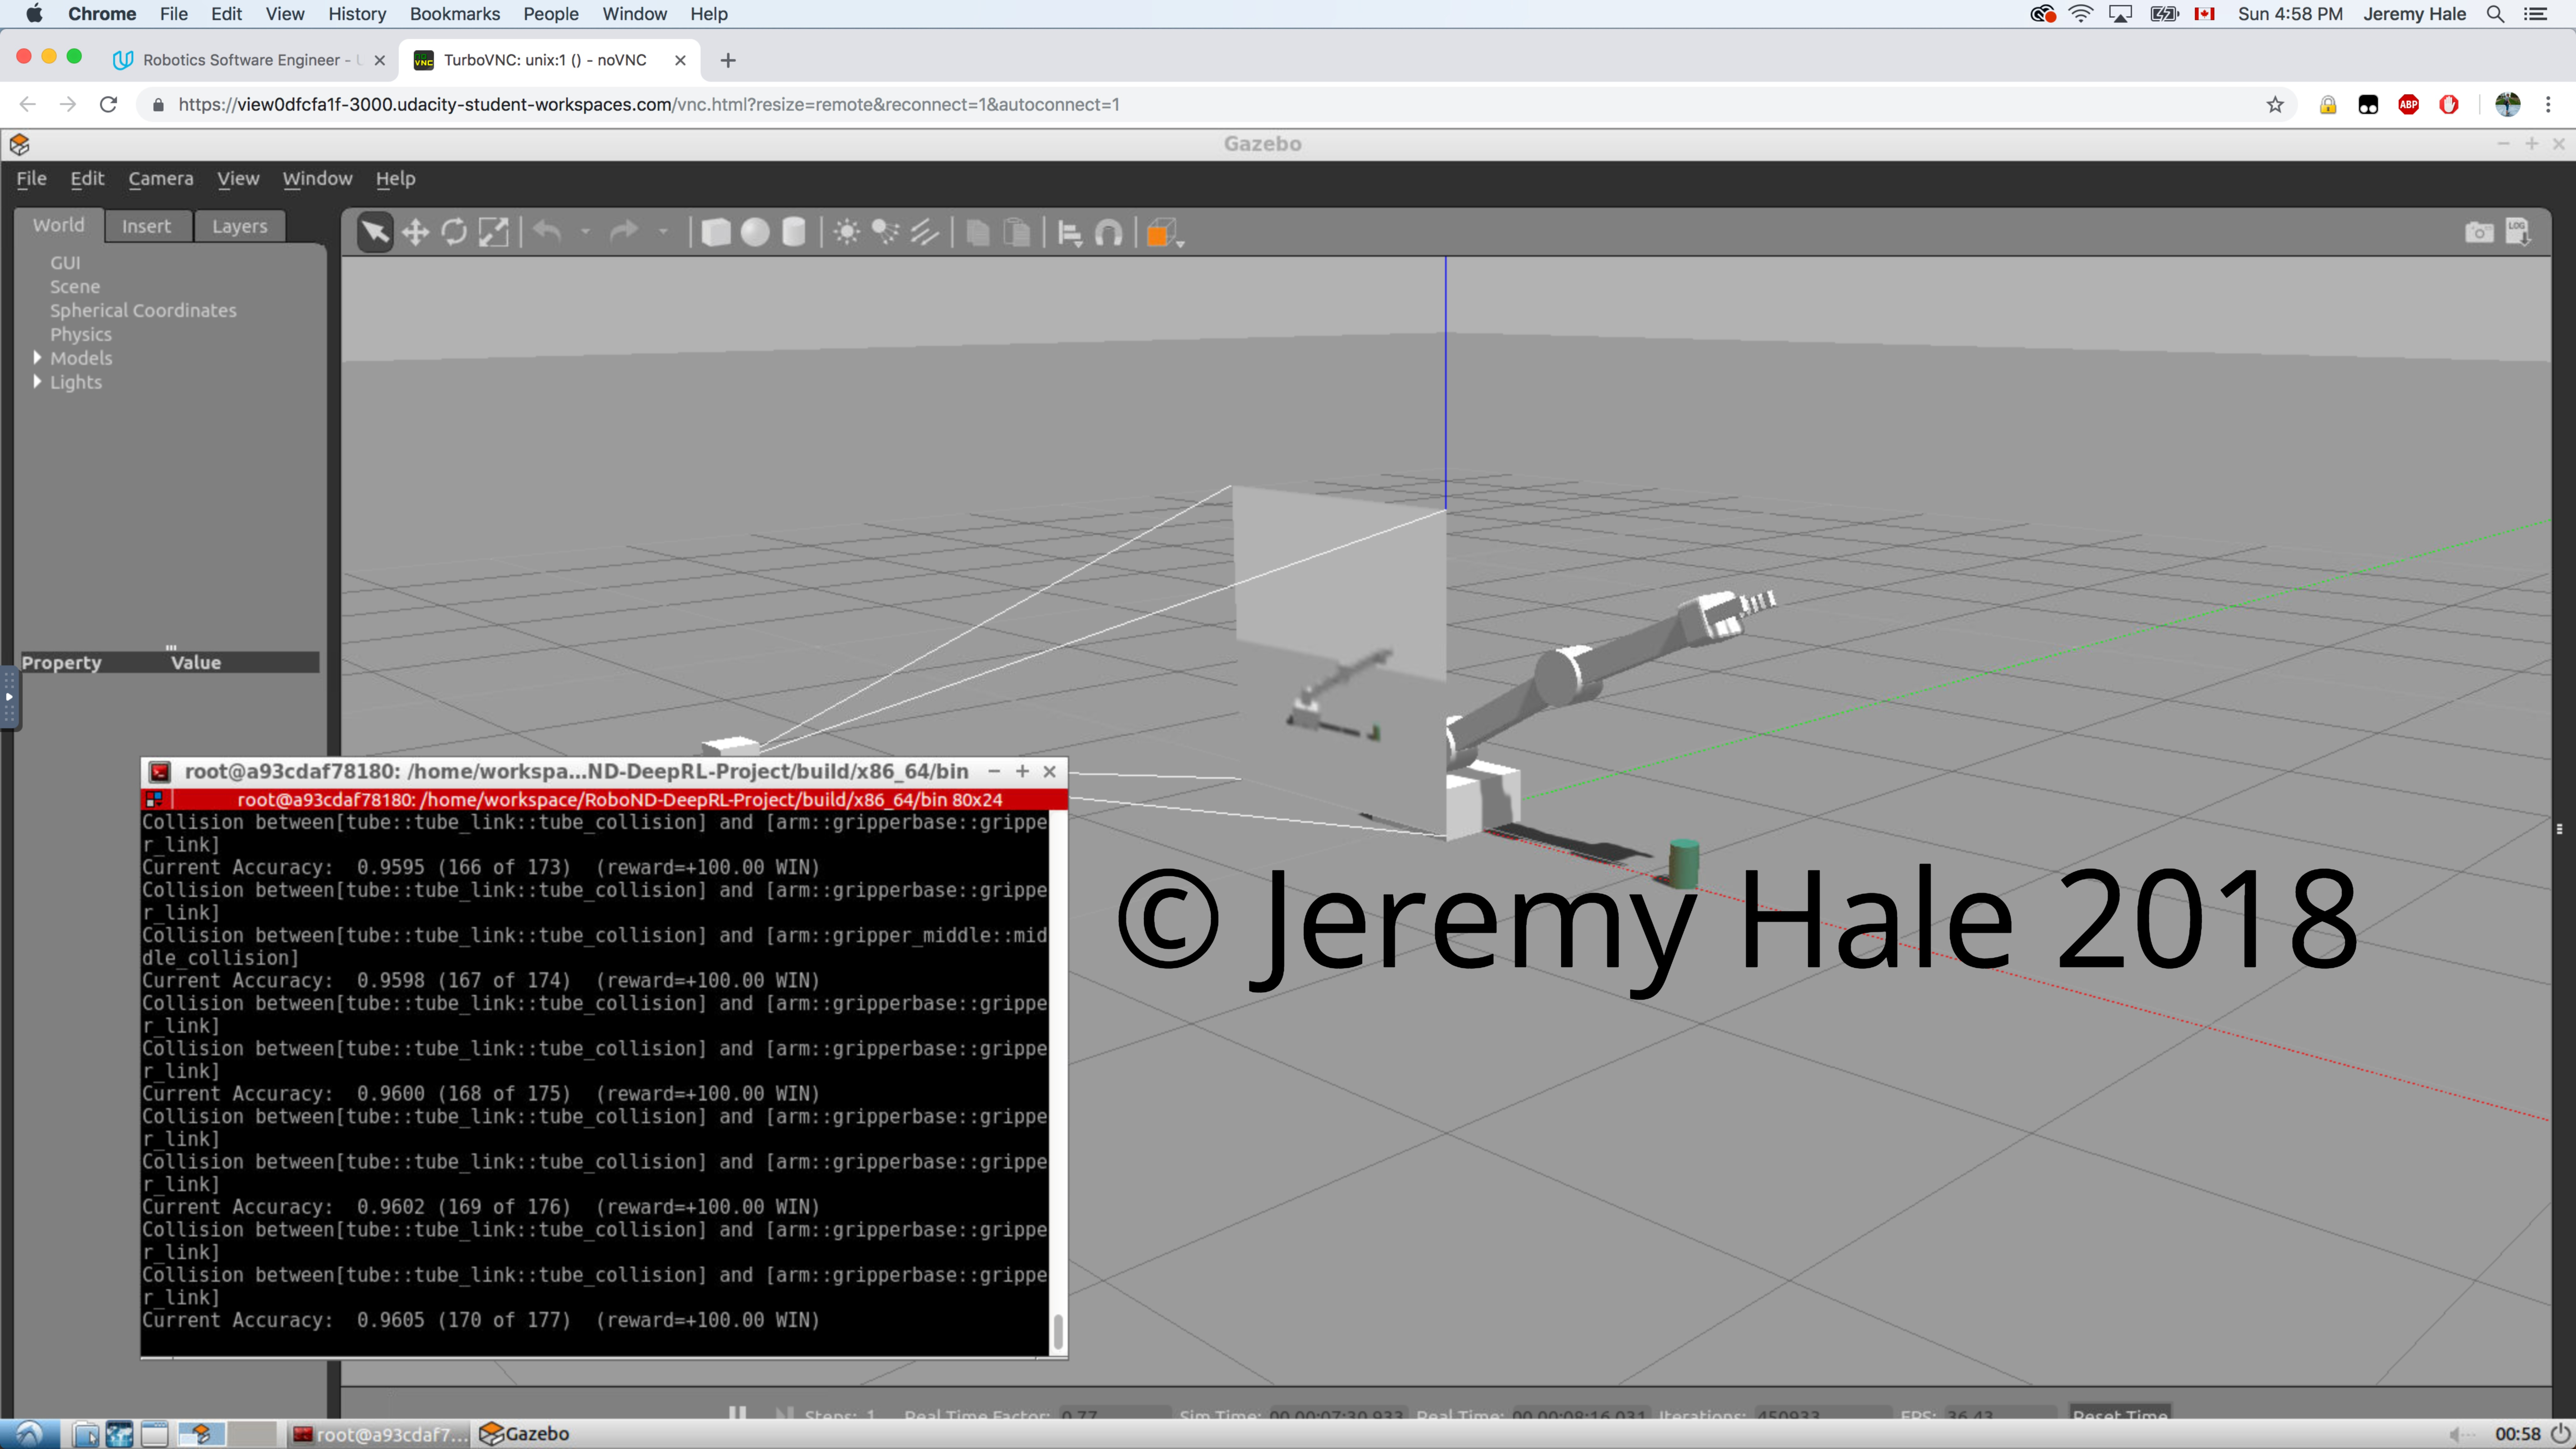
\includegraphics[width=\linewidth]{goal1_water}
    \caption{First Goal}
    \label{fig:first_goal}
\end{figure}

\begin{figure}[thpb]
    \centering
    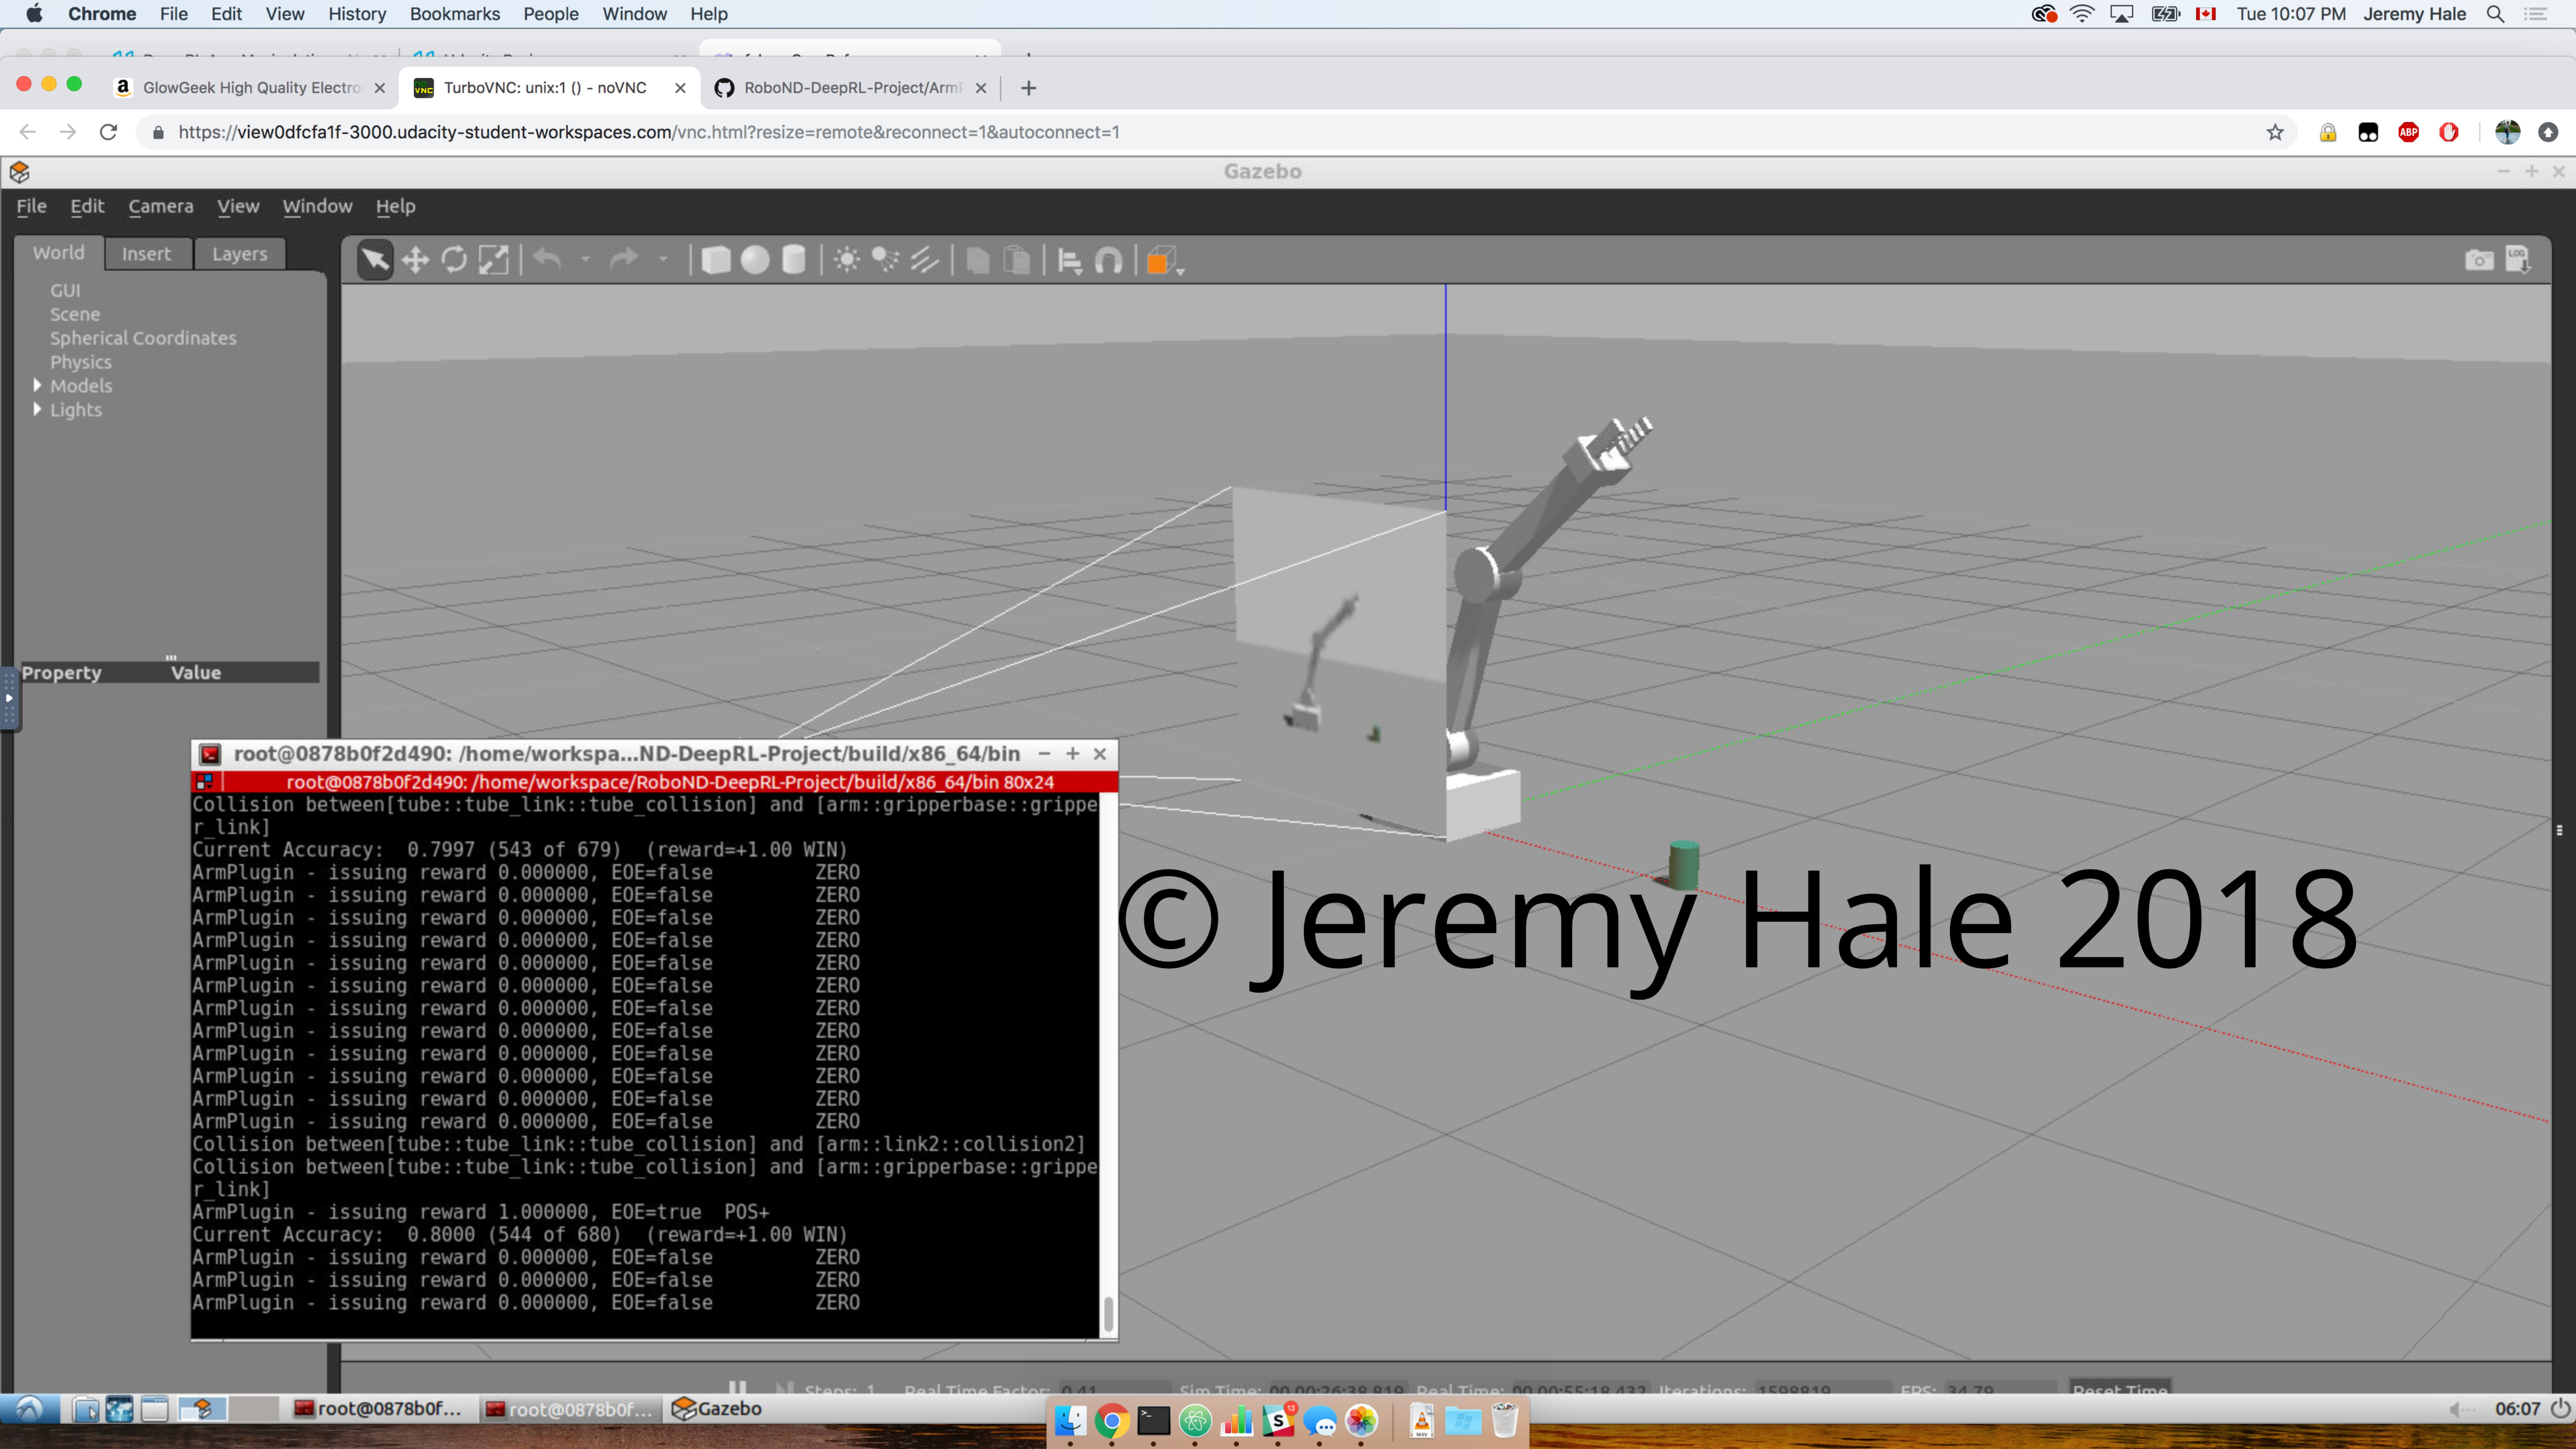
\includegraphics[width=\linewidth]{goal2_water}
    \caption{Second Goal}
    \label{fig:second_goal}
\end{figure}

\section{Future Work}
One of the main difficulties with this task is the lack of repeatability. The speed at which the agent learned seemed fairly random. Sometimes the agent would start to win very quickly other times it would get stuck with some poor behaviour. It is very difficult to improve an algorithm when experiments are not repeatable, so it would be pertinent to explore how the agent is initialized and experiement with randon and deterministic initializations.

Another issue is the time it takes to carry out an experiment. Reducing the episode length helped with this somewhat, but using a different type of agent that can take advantage of more parallel processing would be beneficial.

\end{document}
